% Author: Frantisek Burian
\documentclass{standalone}
\usepackage{tikz}
\usetikzlibrary{arrows, arrows.meta, decorations.markings, shapes, positioning, backgrounds, calc, fit, shapes.geometric}

\tikzstyle{pathelement} = [rectangle, draw, text width=10em, minimum height=1.5em, text centered, line width=0.3mm]

\tikzstyle{vecArrow}[black] = [
    #1,
    thick, 
    double distance=1.4pt, 
    shorten <= -0.85pt,
    arrows={-Triangle[angle=60:7pt,#1,fill=white]},
    postaction = {draw, -, line width = 1.4pt, white, shorten >= 4.0pt, shorten <= 4.0pt}
  ]
\definecolor{chapter-color}{rgb}{.27,.39,.67}
\begin{document}

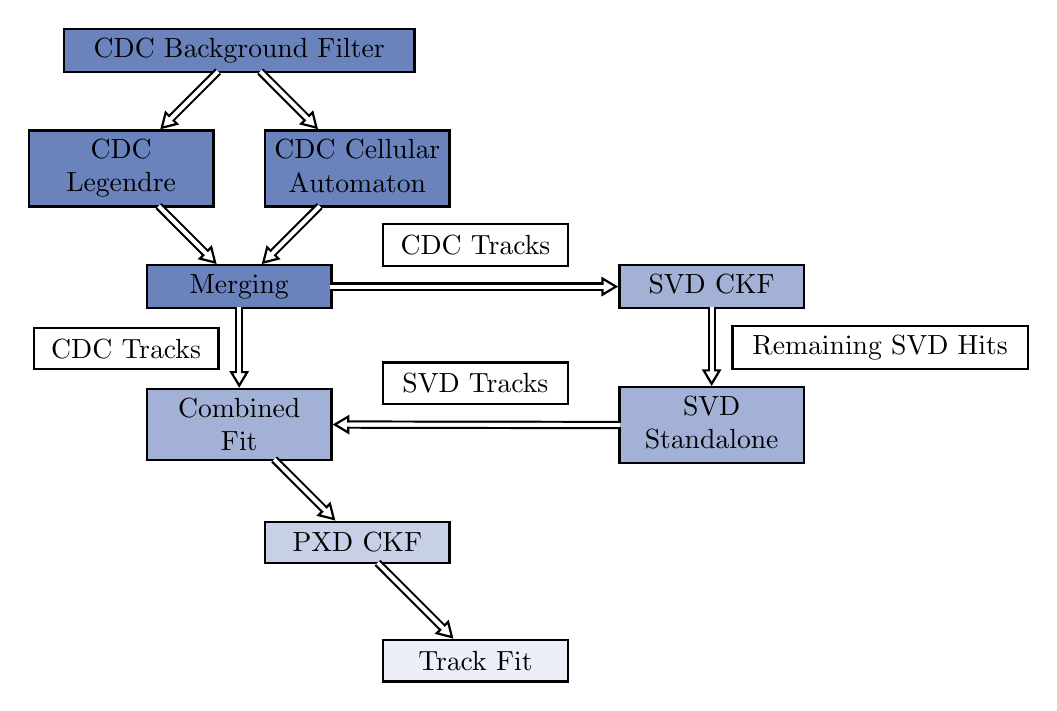
\begin{tikzpicture}
    \node[pathelement, fill=chapter-color!80!white, text width=12em] at (1.5, 1.5) (background) {CDC Background Filter};
    \node[pathelement, fill=chapter-color!80!white, text width=6em] at (0, 0) (legendre) {CDC Legendre};
        \node[pathelement, fill=chapter-color!80!white, text width=6em] at (3, 0) (ca) {CDC Cellular Automaton\vphantom{g}};
        
    \node[pathelement, fill=chapter-color!80!white, text width=6em] at (1.5, -1.5) (merger) {Merging};
        \node[pathelement, fill=chapter-color!50!white, text width=6em] at (7.5, -1.5) (svd_ckf) {SVD CKF\vphantom{g}};

        \node[pathelement, fill=chapter-color!50!white, text width=6em] at (7.5, -3.26) (svd_vxdtf2) {SVD Standalone\vphantom{g}};
        \node[pathelement, fill=chapter-color!50!white, text width=6em] at (1.5, -3.25) (ckf_merger) {Combined Fit};
        
        \node[pathelement, fill=chapter-color!30!white, text width=6em] at (3, -4.75) (pxd) {PXD CKF};
        
    \node[pathelement, fill=chapter-color!10!white, text width=6em] at (4.5, -6.25) (fit) {Track Fit};
        
        \draw[vecArrow] (background) -- (legendre);
        \draw[vecArrow] (background) -- (ca);
        \draw[vecArrow] (legendre) -- (merger);
        \draw[vecArrow] (ca) -- (merger);
        \draw[vecArrow] (merger) -- node[pathelement, above=0.25, midway, text width=6em] {CDC Tracks} (svd_ckf);
        \draw[vecArrow] (svd_ckf) -- node[pathelement, right=0.25, midway, text width=10em] {Remaining SVD Hits} (svd_vxdtf2);
        \draw[vecArrow] (svd_vxdtf2) -- node[pathelement, above=0.25, midway, text width=6em] {SVD Tracks} (ckf_merger);
        \draw[vecArrow] (merger) -- node[pathelement, left=0.25, midway, text width=6em] {CDC Tracks} (ckf_merger);
        \draw[vecArrow] (ckf_merger) -- (pxd);
        \draw[vecArrow] (pxd) -- (fit);
\end{tikzpicture}

\end{document}
